% Foto corregida del diagrama de bloques con zonas funcionales y elementos numerados
\begin{tikzpicture}[
  zona/.style={draw=#1,fill=#1,fill opacity=.07,draw opacity=.9,rounded corners=3pt,
    line width=.9pt,dashed},
  etq/.style={font=\sffamily\scriptsize\bfseries,text=#1,fill=white,draw=#1,
    rounded corners=1.5pt,inner sep=2pt,line width=.6pt},
  guia/.style={#1,line width=.7pt,-{Stealth[length=4pt]}},
  num/.style={circle,fill=navy,text=white,font=\sffamily\bfseries\fontsize{5.5}{6}\selectfont,
    inner sep=0pt,minimum size=9pt,draw=white,line width=.5pt}]
  \node[inner sep=0,anchor=south west] (img) at (0,0)
    {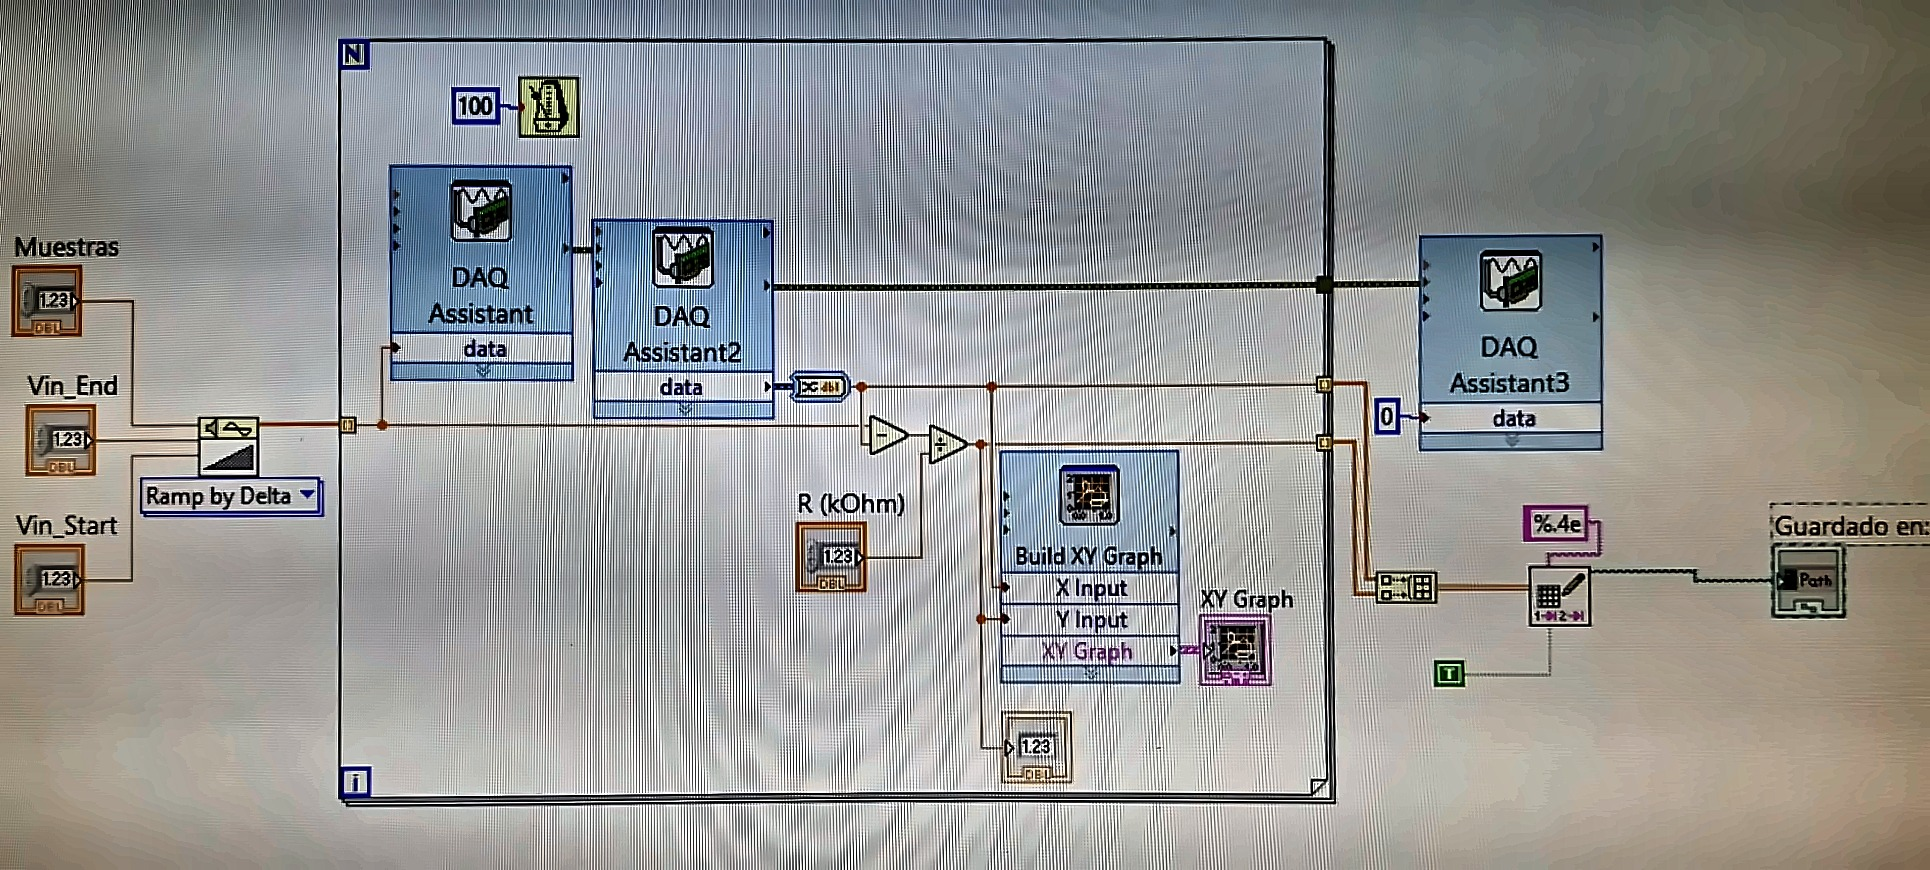
\includegraphics[width=\linewidth]{img/diagrama_bloques.jpg}};
  \begin{scope}[x={(img.south east)},y={(img.north west)}]
    % ---------------- zonas funcionales
    \draw[zona=ambar]     (0.004,0.275) rectangle (0.172,0.765);
    \draw[zona=grisazul]  (0.226,0.835) rectangle (0.322,0.93);
    \draw[zona=cRojo]     (0.218,0.545) rectangle (0.320,0.825);
    \draw[zona=cAzul]     (0.324,0.505) rectangle (0.418,0.785);
    \draw[zona=cVerde]    (0.412,0.305) rectangle (0.522,0.630);
    \draw[zona=cUV]       (0.524,0.085) rectangle (0.688,0.495);
    \draw[zona=cRojo]     (0.700,0.455) rectangle (0.842,0.745);
    \draw[zona=navy]      (0.700,0.175) rectangle (0.995,0.445);
    % ---------------- etiquetas de zona (fuera de la foto)
    \node[etq=ambar,anchor=south] (z1) at (0.085,1.035) {A\ \ Rampa de $V_{\text{in}}$};
    \draw[guia=ambar] (z1.south) -- (0.085,0.765);
    \node[etq=grisazul,anchor=south] (z2) at (0.255,1.035) {B\ \ Temporización};
    \draw[guia=grisazul] (z2.south) -- (0.27,0.93);
    \node[etq=cRojo,anchor=south] (z3) at (0.395,1.035) {C\ \ Salida AO-0};
    \draw[guia=cRojo] (z3.south) -- (0.30,0.825);
    \node[etq=cAzul,anchor=south] (z4) at (0.53,1.035) {D\ \ Adquisición AI-1};
    \draw[guia=cAzul] (z4.south) -- (0.40,0.785);
    \node[etq=cRojo,anchor=south] (z7) at (0.78,1.035) {G\ \ Reinicio AO-0 $=0$\,V};
    \draw[guia=cRojo] (z7.south) -- (0.78,0.745);
    \node[etq=grisazul,anchor=north] (zf) at (0.24,-0.04) {Bucle \ttt{For}: una medida por iteración};
    \draw[guia=grisazul] (zf.north) -- (0.24,0.07);
    \node[etq=cVerde,anchor=north] (z5) at (0.47,-0.04) {E\ \ Cálculo de $I_D$};
    \draw[guia=cVerde] (z5.north) -- (0.47,0.305);
    \node[etq=cUV,anchor=north] (z6) at (0.63,-0.04) {F\ \ Representación};
    \draw[guia=cUV] (z6.north) -- (0.63,0.085);
    \node[etq=navy,anchor=north] (z8) at (0.85,-0.04) {H\ \ Guardado en fichero};
    \draw[guia=navy] (z8.north) -- (0.85,0.175);
    % ---------------- elementos numerados
    \foreach \n/\x/\y in {1/0.072/0.700, 2/0.077/0.548, 3/0.072/0.385, 4/0.122/0.590,
        5/0.163/0.585, 6/0.214/0.940, 7/0.214/0.100, 8/0.233/0.812, 9/0.312/0.880,
        10/0.229/0.795, 11/0.333/0.757, 12/0.432/0.612, 13/0.455/0.445, 14/0.508/0.540,
        15/0.404/0.330, 16/0.536/0.472, 17/0.668/0.228, 18/0.566/0.118, 19/0.600/0.705,
        20/0.670/0.585, 21/0.748/0.722, 22/0.711/0.470, 23/0.722/0.385, 24/0.838/0.290,
        25/0.783/0.440, 26/0.776/0.228, 27/0.905/0.270}
      \node[num] at (\x,\y) {\n};
  \end{scope}
\end{tikzpicture}
